
\begin{figure*}[tp!]
   \centering
   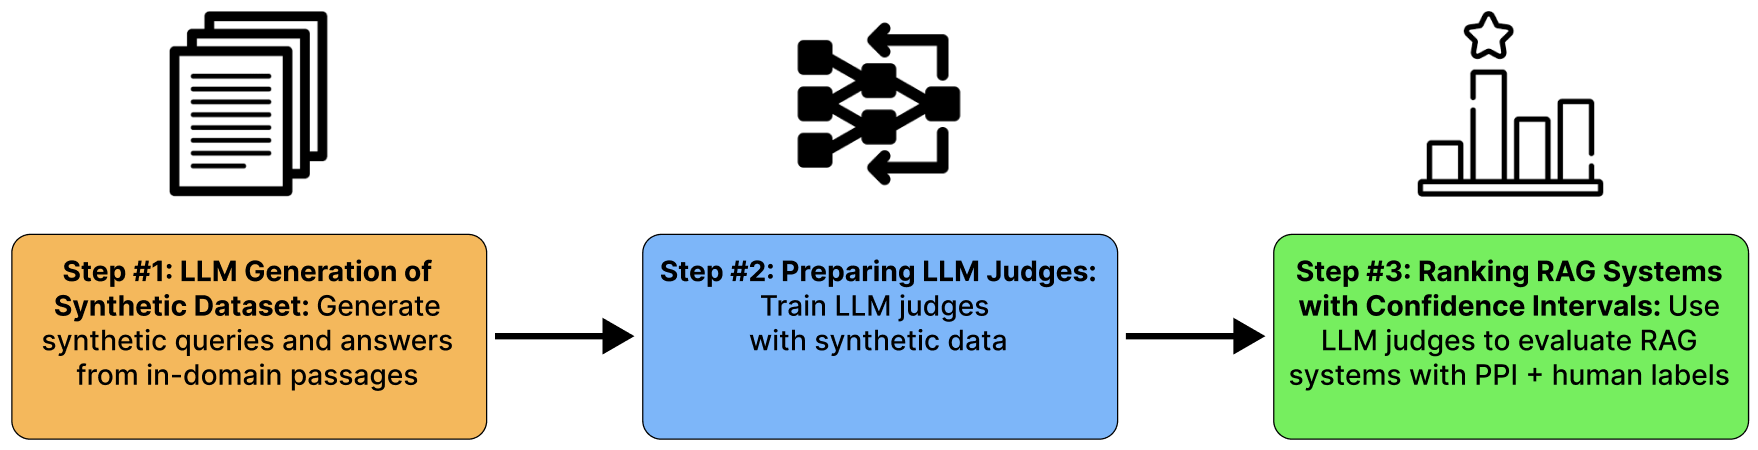
\includegraphics[width=0.9\linewidth]{Tables/Headline_Figure_V1.png}
   \caption{\textbf{Overview of ARES}:
   As inputs, the ARES pipeline requires an in-domain passage set, a human preference validation set of 150 annotated datapoints or more, and few-shot examples of in-domain queries and answers (five or more), which are used for prompting LLMs in synthetic data generation.
   To prepare our LLM judges for evaluation, we first generate synthetic queries and answers from the corpus passages. 
   Using our generated training triples and a constrastive learning framework, we fine-tune an LLM to classify query--passage--answer triples in three different criteria: context relevance, answer faithfulness, and answer relevance.
   Finally, we use the LLM judges to score RAG systems and generate confidence bounds for the ranking using PPI and the human preference validation set. 
   }
   \label{fig:domain_adaptation_diagram}
\end{figure*}
